\documentclass[aspectratio=169]{beamer}

\usetheme{Boadilla}
%\usetheme{I6pd2}
\usecolortheme[light,accent=violet]{solarizedJMK}

\usepackage{comment}
\usepackage{graphicx}
\graphicspath{{../doc/},{../doc/figs/},{../Nest/doc/},{doc/},{../writeups/doc/},{../writeups/},{./doc/}}
\usepackage[absolute,overlay]{textpos}
  \setlength{\TPHorizModule}{1in}
  \setlength{\TPVertModule}{1in}
\usepackage{tikz}
\usepackage{natbib}
\usepackage{multimedia}
\usepackage{adjustbox}


\usetikzlibrary{arrows,shapes,backgrounds}

% \usepackage{beamerthemesplit} // Activate for custom appearance

\title[TTide SIO 2015]{Tasmania internal tide experiment: Preliminary modeling}
\subtitle{}
\author{Jody Klymak}
\institute[UVic]{University of Victoria}
\date{\today}

\setbeamercovered{highly dynamic}

\defbeamertemplate*{title page}{customized}[1][]
{
  	\usebeamerfont{title}\inserttitle\par
  	\usebeamerfont{subtitle}\usebeamercolor[fg]{subtitle}\insertsubtitle\par
   	\bigskip
  	\usebeamerfont{author}\insertauthor\par
  	\usebeamerfont{institute}\insertinstitute\par
  	\usebeamerfont{date}\insertdate\par
	\bigskip
  \begin{center}
 	 	\usebeamercolor[fg]{titlegraphic}\inserttitlegraphic
   \end{center}
 	\usebeamerfont{author}Rob Pinkel,  Matthew Alford, Jennifer MacKinnon, Jonathan Nash, Harper Simmons, Dmitry Brazhnikov, Sam Kelly, Amy Waterhouse, Nicole Jones\par	 
}

\titlegraphic{\includegraphics[width=.9\textwidth]{Klymaketal12Fig1.pdf}}

%\usebackgroundtemplate{%
%  
\includegraphics[width=\paperwidth,height=\paperheight,angle=0,trim=0 15 0 0,clip]{doc/TurbBlur.png}} 

\begin{comment}
Points:
- Goal: how "reflective" is this slope
- Tasman Rise diffracts:
  - I don't know what is coming in because of diffraction
  - two moorings and plane/wave fits difficult (must make scale of fits small enough).
- Simple 2-D reflection over predicts reflectivity of whole.
- Super-inertial slope wave is strummed that redistributes energy along-slope

\end{comment}

 

\begin{document}

\frame{\titlepage}

%\section[Outline]{}
%\frame{\tableofcontents}
\begin{comment}
\end{comment}

\section{Intro and Motivation}
\def\tikzoverlay{%
   \tikz[baseline,overlay]\node[every overlay node]
}%

\tikzset{thick arc/.style={->, black, fill=none, ultra thick, >=stealth, text=black}}

\tikzstyle{background grid}=[draw, black!50,step=.5cm]

\begin{frame}
  \frametitle{Experiment Goal}
  \framesubtitle{Turbulence due to continental slope}
  \includegraphics<1>[width=0.9\textwidth,trim=0 0 0 0, clip]{../writeups/Time11Annote.png}
  \includegraphics<2>[width=0.9\textwidth,trim=0 0 0 0, clip]{../writeups/Time11Annote2.png}
  
  \begin{itemize}
    \item<1->Parameterize dissipation, $D=F_{in}-F{out}$ as function of $F_{in}$ (not trivial).
    \item<2->But more basic: how to disentangle $F_{in}$ from $F_{net}$?  
  \end{itemize}
\end{frame}

\begin{frame}
  \frametitle{TTide: Tasmania Internal Tide Experiment}
  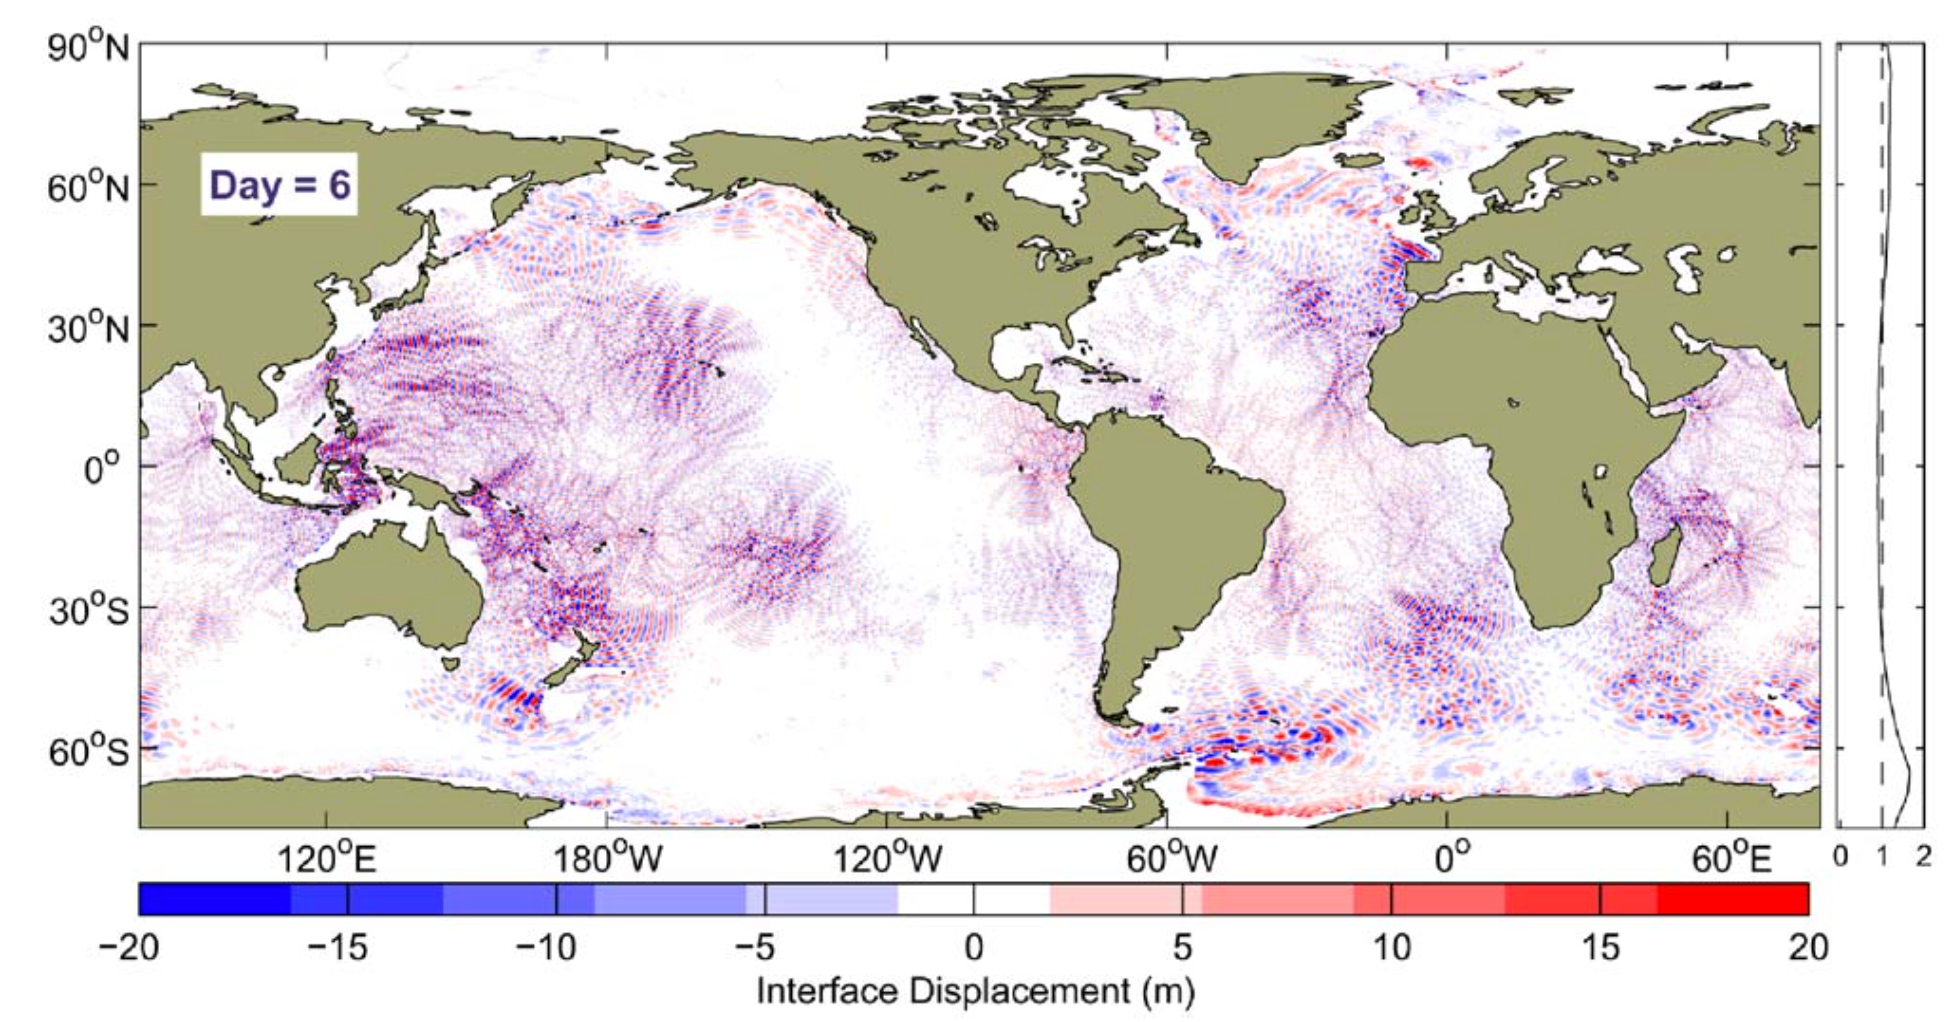
\includegraphics[width=0.9\textwidth]{doc/SimmonsEtAl04a.png}
  
  \emph{Simmons et al 2004}
\end{frame}

\begin{frame}
  \frametitle{TTide: Tasmania Internal Tide Experiment}
  \begin{center}
  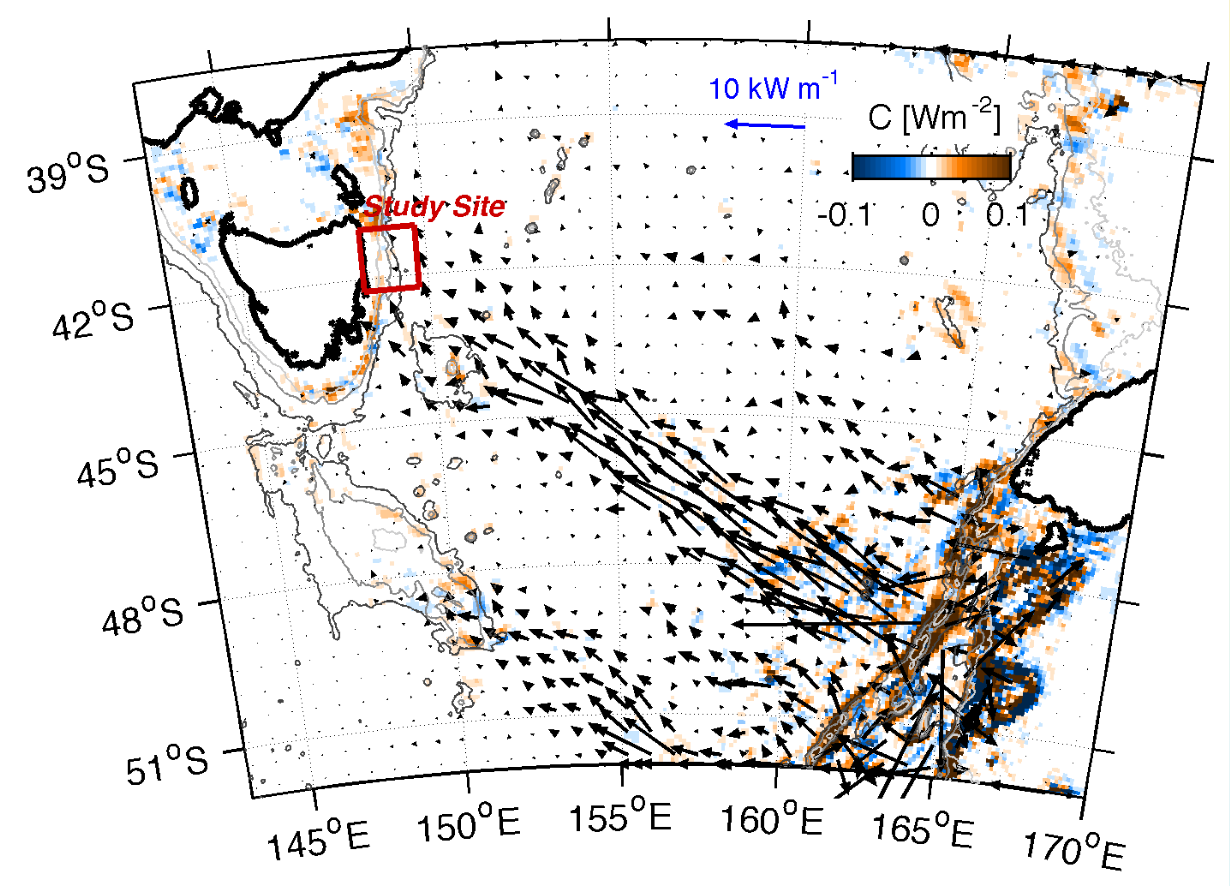
\includegraphics[width=0.7\textwidth]{doc/SiteMap.png}
  \end{center}
  \emph{Simmons et al 2004}
\end{frame}

\begin{frame}
  \frametitle{TTide: Tasmania Internal Tide Experiment}
  \begin{center}
  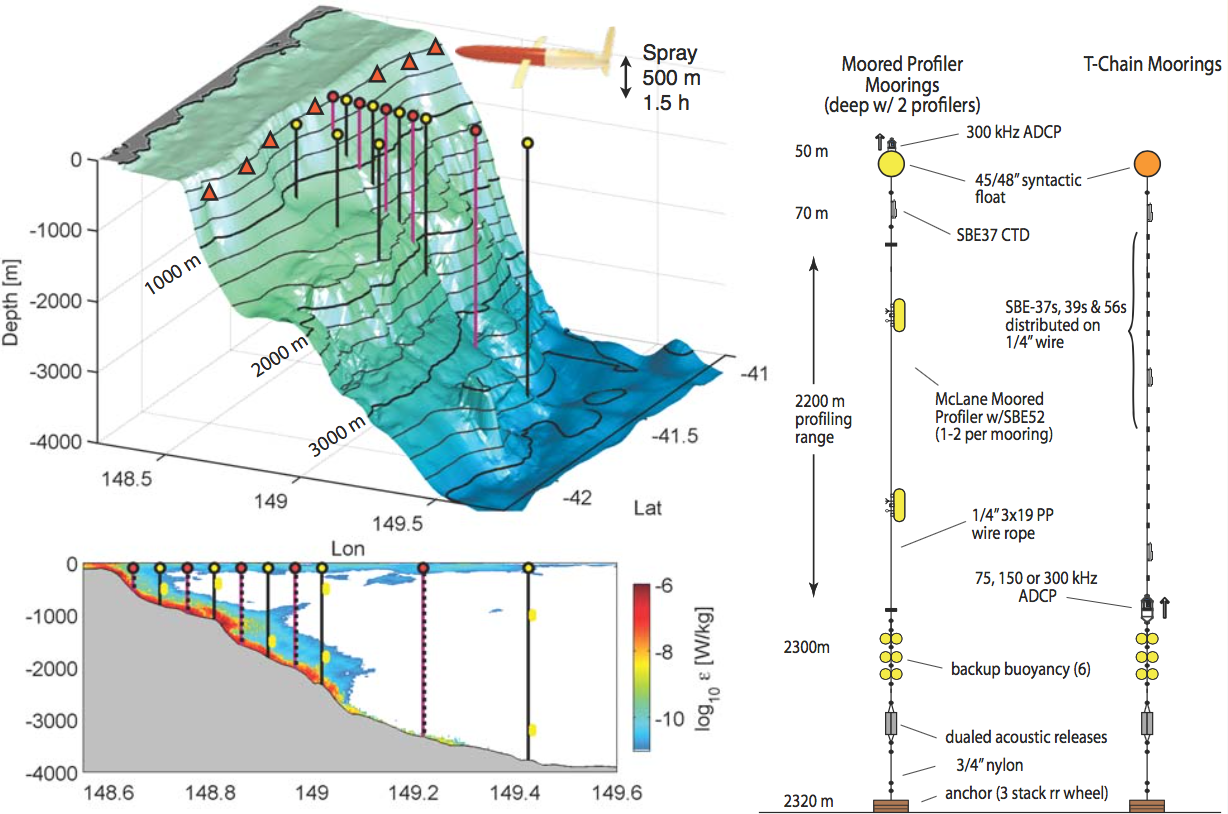
\includegraphics[width=0.7\textwidth]{doc/ExperimentSketch.png}
  \end{center}
\end{frame}


\section{Setup}
\frame{\frametitle{Setup}
  \begin{center}
   \includegraphics<1>[width=0.95\textwidth,trim=0 0 0 0, clip]{doc/AnalyticalForcing}
  \end{center}
      \begin{itemize}
        \item<1> MITgcm (hydrostatic, Klymak and Legg 2010 dissipation) 
        \item<1> Analytical $M_2$, mode-1, forcing meant to represent Macquarie Ridge
        \item<1> Central region 1 km x 1 km, telescope around this.
        \item<1> sponge forcing and absorbers 
      \end{itemize}
}% end frame
\frame{\frametitle{Simple Response?}
  \begin{center}
   \includegraphics<1>[width=0.95\textwidth,trim=0 0 0 0, clip]{doc/AnalyticalForcing}
  \end{center}
      \begin{itemize}
        \item<1> Standing wave cross-slope ($k_x=cos(30)k_r$)
        \begin{itemize}
            \item<1> beam at about 30 degrees to wall.
            \item<1> 180 degree phase reversal at 50 km, 150 km, 250 km etc.
        \end{itemize}
        \item<1> Propagating wave along-slope ($k_y=sin(30)k_r$)
        \item<1> Slight curvature due to the spherical spreading of the incoming wave.
      \end{itemize}
}% end frame

%%%%%%%%%%%%%%%%%%%%%%%%%%%
\section{Response}
%%%%%%%%%%%%%%%%%%%%%%%%%%%

\frame{\frametitle{Response}
\framesubtitle{MITgcm; realistic bathymetry}
\framesubtitle<2>{Energy Budget (Depth-integrated; tidally averaged)}
\begin{center}
  \includegraphics<1>[width=0.65\textwidth,trim=0 0 0 0, clip]{doc/VelFluxReal1km03.pdf}
  \includegraphics<2>[width=0.8\textwidth,trim=0 0 0 0, clip]{doc/DissReal1km03cycle20.pdf} 
\end{center}
}

\frame{\frametitle{Net Energy Budget}
\begin{columns}
  \begin{column}{0.6\textwidth}
    \includegraphics[width=\textwidth,trim=0 0 0 0, clip]{./doc/DissReal1km03cycle20.pdf} 
  \end{column}
  \begin{column}{0.4\textwidth}
    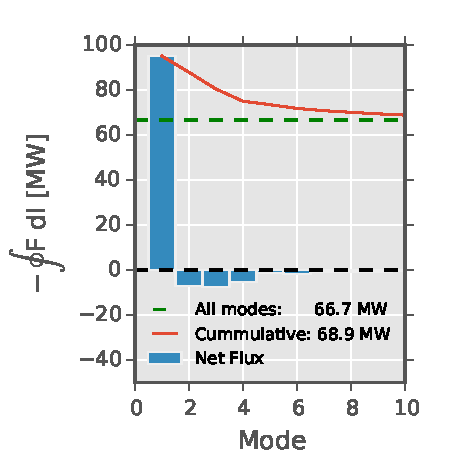
\includegraphics[width=\textwidth]{./doc/RealEnergyFluxModesSum.pdf}
  \end{column}
\end{columns}
}

\begin{frame}
  \frametitle{Points}
  \begin{columns}
    \begin{column}{0.4\textwidth}
      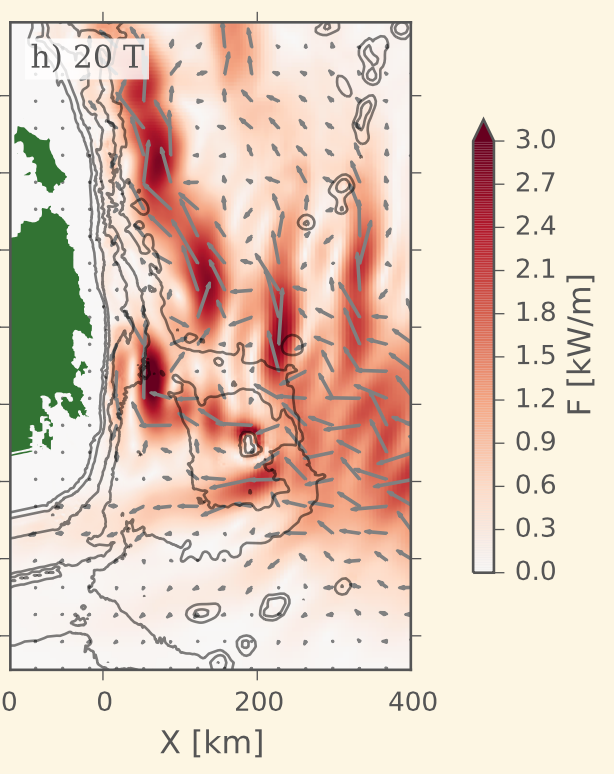
\includegraphics[width=\textwidth]{doc/Tide20Full.png}
      
    \end{column}
    \begin{column}{0.5\textwidth}
      \begin{itemize}
        \item<1-> Tasman Rise diffracts incoming energy
          \begin{itemize}
             \item<1-> Localized energy: hard to do plane-wave fits
             \item<1-> We don't \emph{know} what the incoming flux is
          \end{itemize}
        \item<2-> Reflectivity is somewhat less than 2-D reflectivity estimates
        \item<3-> There is a strong super-inertial BT/BC slope wave that redistributes energy along shelf.
      \end{itemize}
    \end{column}
  \end{columns}
\end{frame}

\section{Two Wave Fit}

\frame{\frametitle{Two-waves: mooring}
\begin{columns}
  \begin{column}{0.55\textwidth}
    \begin{center}
      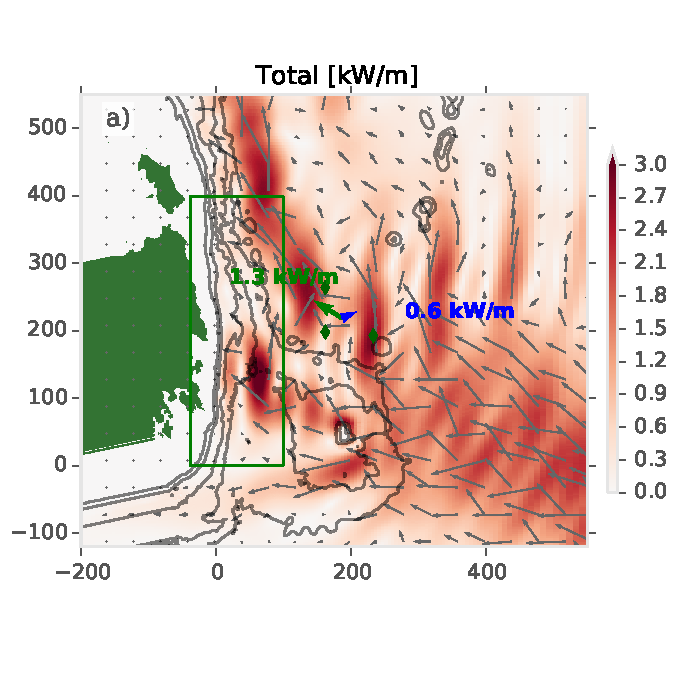
\includegraphics[width=0.99\textwidth,trim=0 0 0 0, clip]{doc/TwoWaves.pdf}\\ 
    \end{center}
    
  \end{column}
  \begin{column}{0.5\textwidth}
    \begin{itemize}
      \item Two-wave plane fit
      \item $F_{in}=1.3\ kW/m$, $F_{out}=0.6\ kW/m$
      \item $D>0.5 F_{in}$!
      \item Do we believe this (hint: no, below we will show $D\approx 0.25 F_{in}$). 
    \end{itemize}  
  \end{column}
\end{columns}
}

\section{Splitting the waves in model}

\frame{\frametitle{Incoming versus outgoing: Simplified Geometries}
\begin{center}
  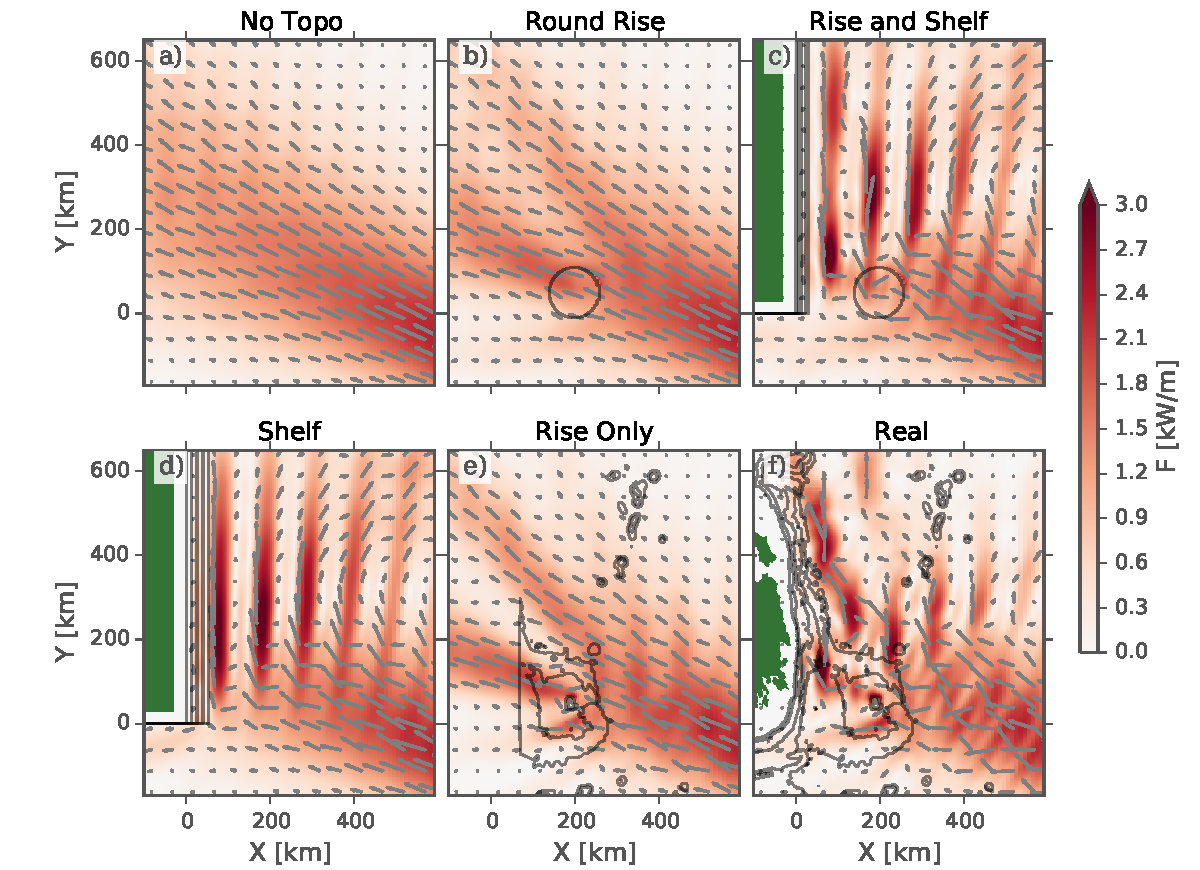
\includegraphics[width=0.65\textwidth]{./doc/EnergyFluxesAll.pdf}
\end{center}
} %\end frame

\frame{\frametitle{Incoming versus outgoing: Simple Shelf}
\begin{center}
  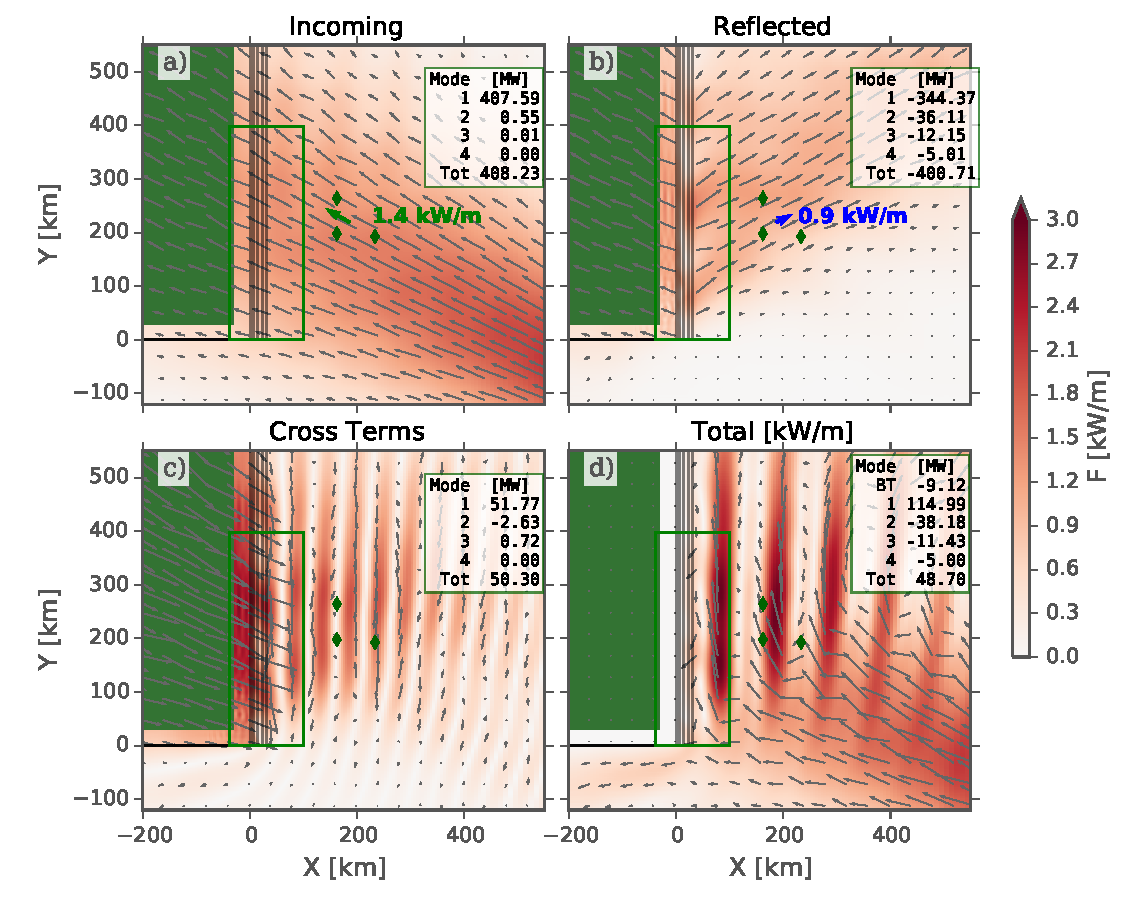
\includegraphics[width=0.6\textwidth]{./doc/ShelfResponseMode1.pdf}
\end{center}
} %\end frame

\frame{\frametitle{Incoming vs Outgoing}
\begin{columns}
  \begin{column}{0.45\textwidth}
    \begin{center}
  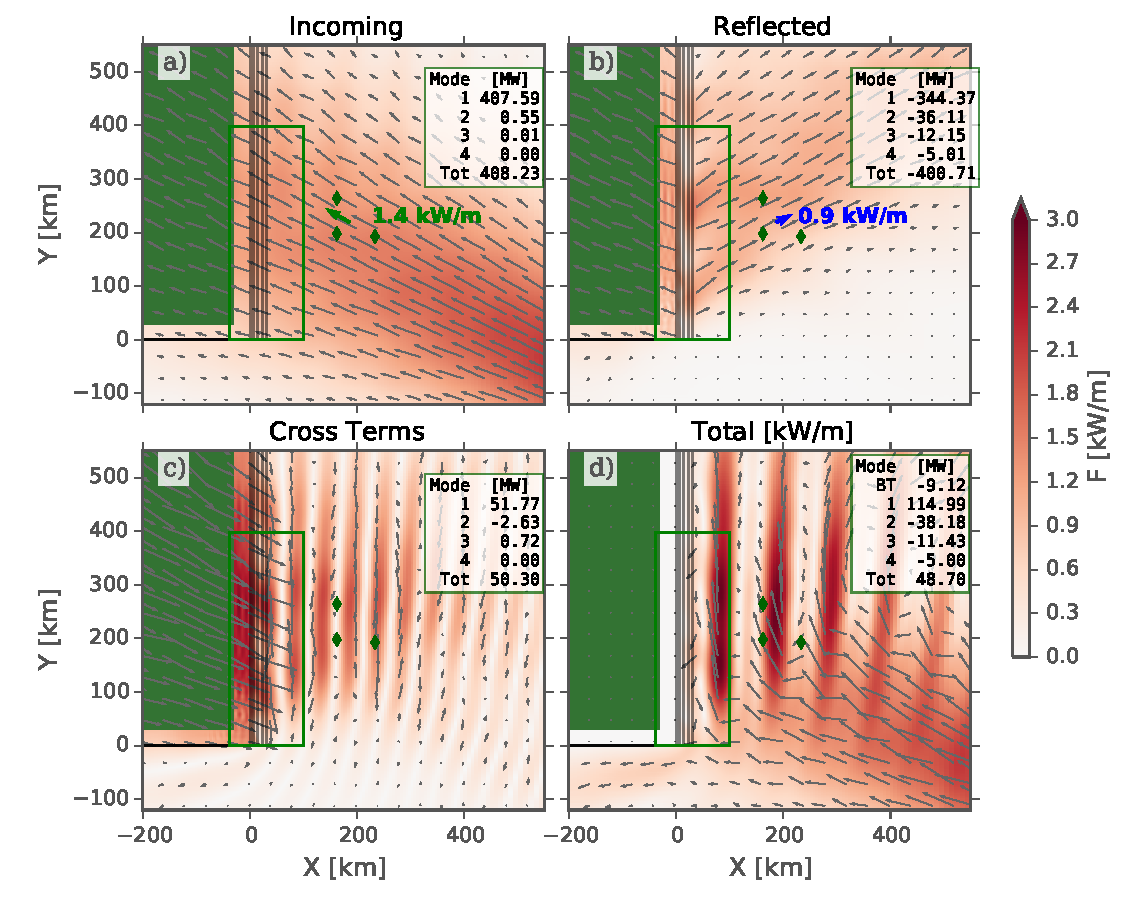
\includegraphics[width=0.99\textwidth]{./doc/ShelfResponseMode1.pdf}
\end{center}
  \end{column}
  \begin{column}{0.55\textwidth}
  \small 
    \begin{eqnarray*}
  u_{1}^{t}(x,y) &= &u_{1}^{i}+u_{1}^{r}\\
  v_{1}^{t}(x,y) &= &v_{1}^{i}+v_{1}^{r}\\
  p_{1}^{t}(x,y) &= &p_{1}^{i}+p_{1}^{r}
\end{eqnarray*}
\begin{eqnarray*}
  P_{u1}^t & = & \overbrace{u_1^ip_1^i}^{Incoming} + \overbrace{u_1^rp_1^r}^{Reflected} + 
  \overbrace{u_1^ip_1^r + u_1^rp_1^i}^{Cross\ Terms} \\
  P_{v1}^t & = & \overbrace{v_1^ip_1^i}^{Incoming} + \overbrace{v_1^rp_1^r}^{Reflected} + 
  \overbrace{v_1^ip_1^r + v_1^rp_1^i}^{Cross\ Terms} 
\end{eqnarray*}
  \end{column}
\end{columns}
} %\end frame

\frame{\frametitle{Incoming vs Outgoing: Simple shelf}
\begin{columns}
  \begin{column}{0.65\textwidth}
    \begin{center}
      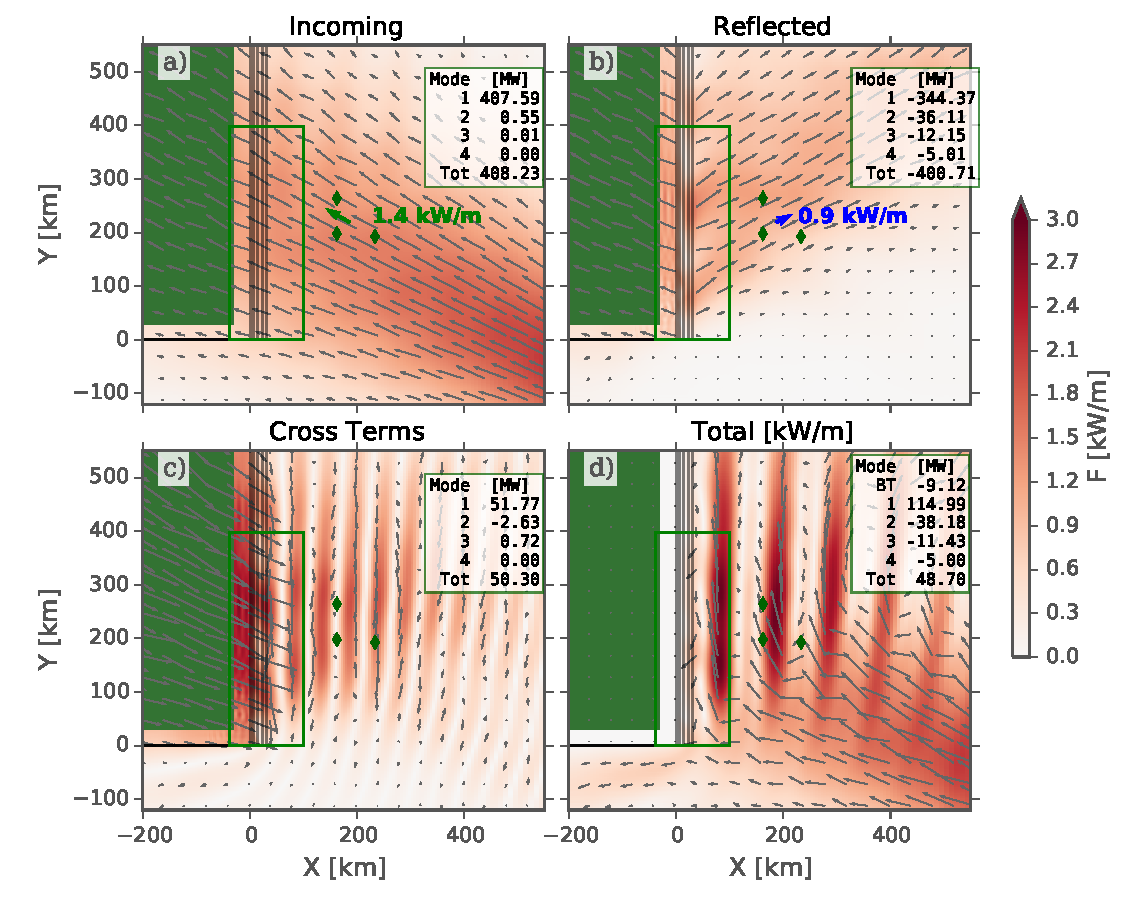
\includegraphics[width=\textwidth]{./doc/ShelfResponseMode1.pdf}
    \end{center}
  \end{column}

  \begin{column}{0.35\textwidth}
    \begin{itemize}
      \item In:    +408 MW
      \item Cross: + 50 MW
      \item Out:   -400 MW
      \item Diss:   50  MW = 11\%
    \end{itemize}
        \vspace{2em}
    \footnotesize{
      (Note: slight energy imbalance -- 58 vs 50 MW -- because ``Incoming'' energy fluxes are inaccurate over shelf.)}
  \end{column}
\end{columns}
} %\end frame

%\frame{\frametitle{Incoming vs Outgoing: Simple Rise and Shelf}
%\begin{center}
%  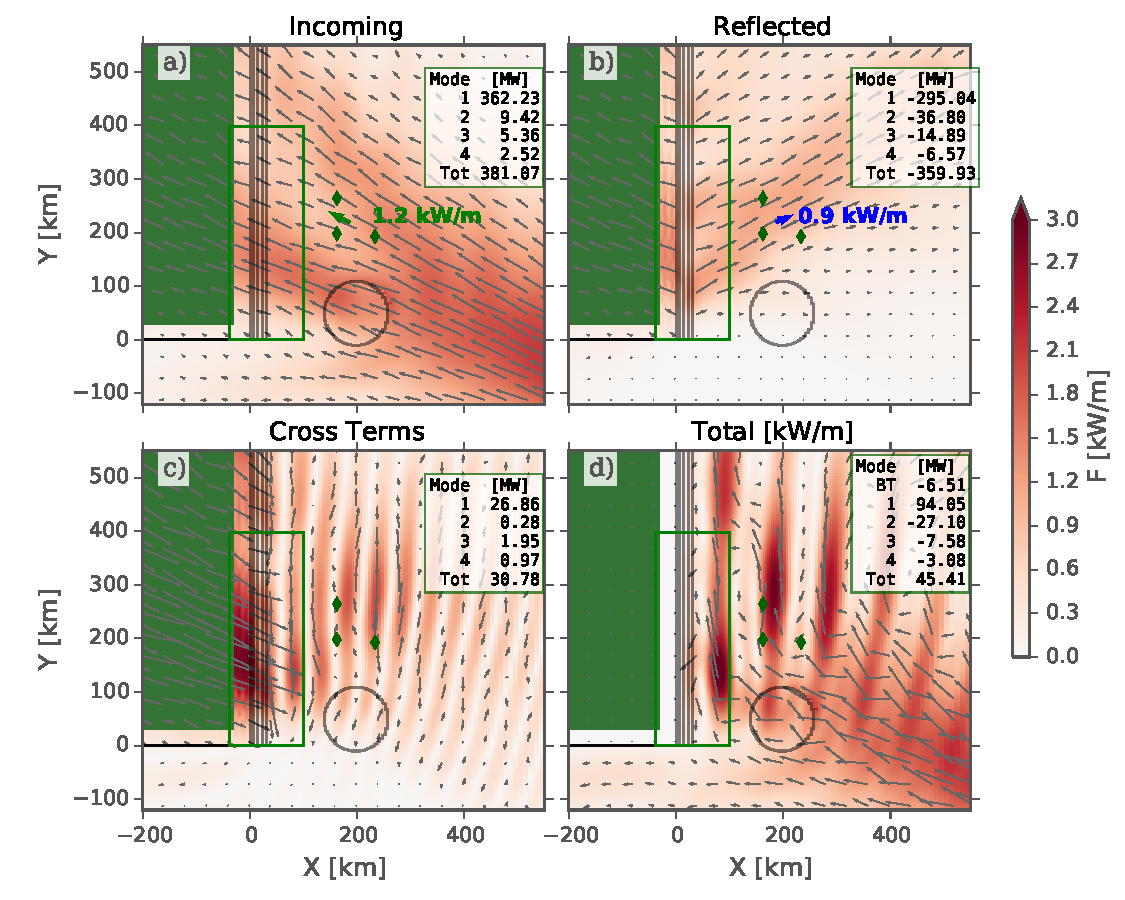
\includegraphics[width=0.62\textwidth]{./doc/RiseShelfResponseMode1.pdf}
%\end{center}
%} %\end frame
%
%\frame{\frametitle{Incoming vs Outgoing: Simple Rise and Shelf}
%\begin{columns}
%  \begin{column}{0.65\textwidth}
%    \begin{center}
%      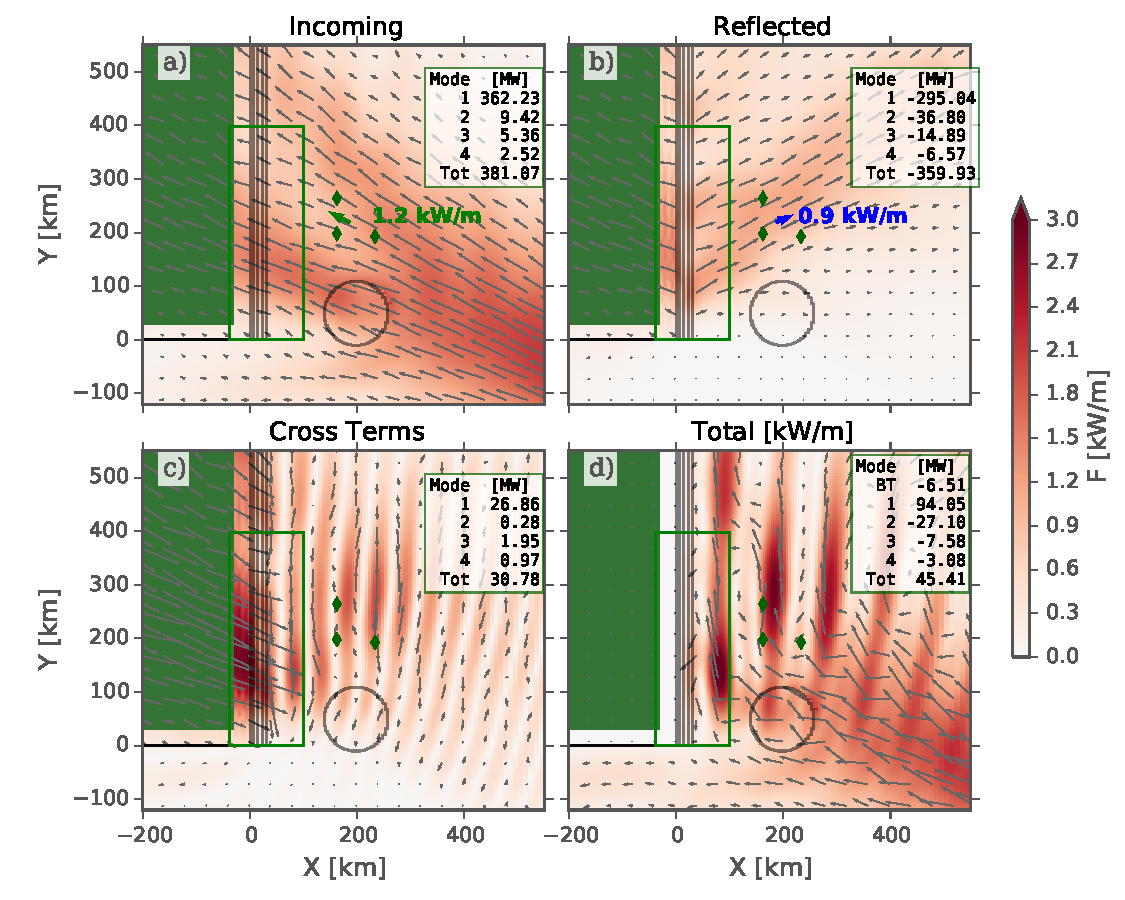
\includegraphics[width=\textwidth]{./doc/RiseShelfResponseMode1.pdf}
%    \end{center}
%  \end{column}
%
%  \begin{column}{0.35\textwidth}
%    \begin{itemize}
%      \item In:    +381 MW
%      \item Cross: + 31 MW
%      \item Out:   -360 MW
%      \item Diss:    45 MW = 11\%
%    \end{itemize}
%    
%    \vspace{2em}
%    \footnotesize{
%      (Note: slight energy imbalance -- 52 vs 45 MW -- because ``Incoming'' energy fluxes are inaccurate over shelf.)}
%  \end{column}
%
%\end{columns}
%} %\end frame


\frame{\frametitle{Incoming vs Outgoing: Realistic}
\begin{center}
  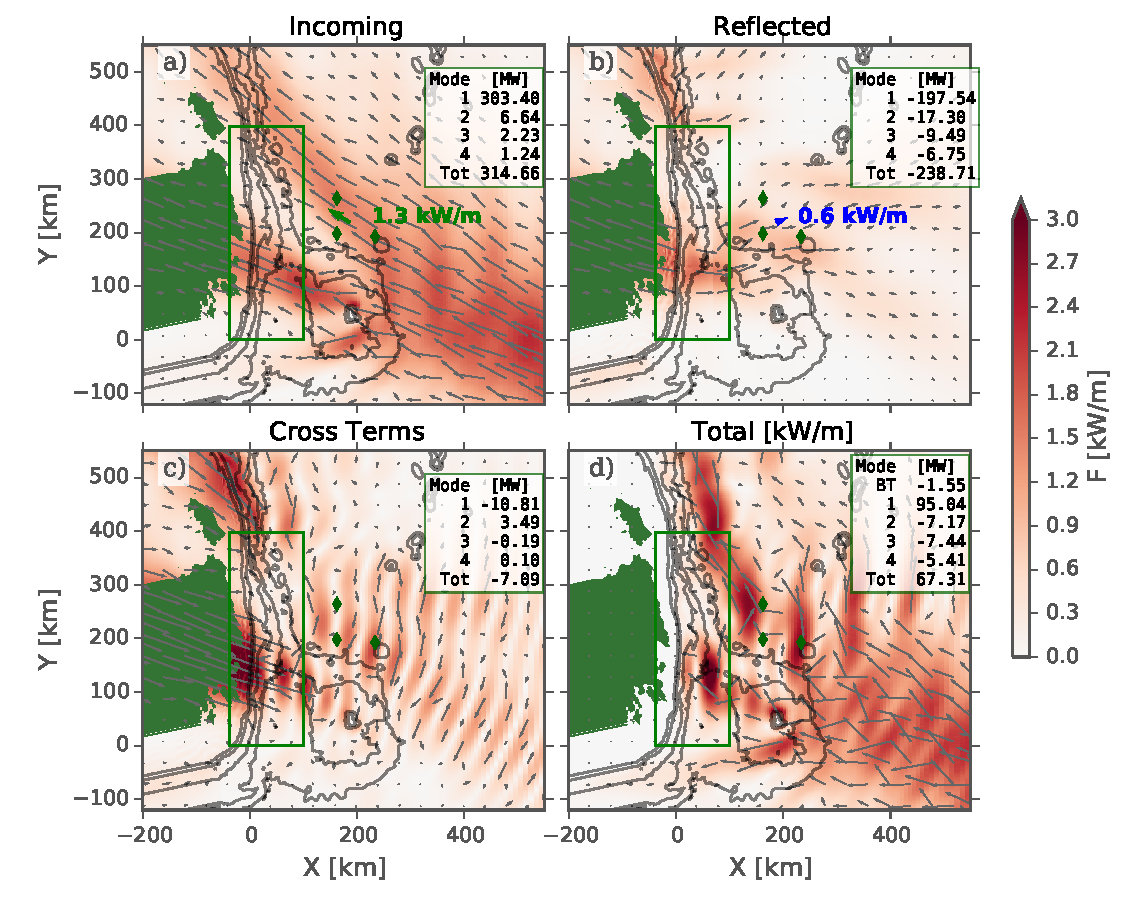
\includegraphics[width=0.62\textwidth]{./doc/RealResponseMode1.pdf}
\end{center}
} %\end frame

\frame{\frametitle{Incoming vs Outgoing: Realistic}
\begin{columns}
  \begin{column}{0.65\textwidth}
    \begin{center}
      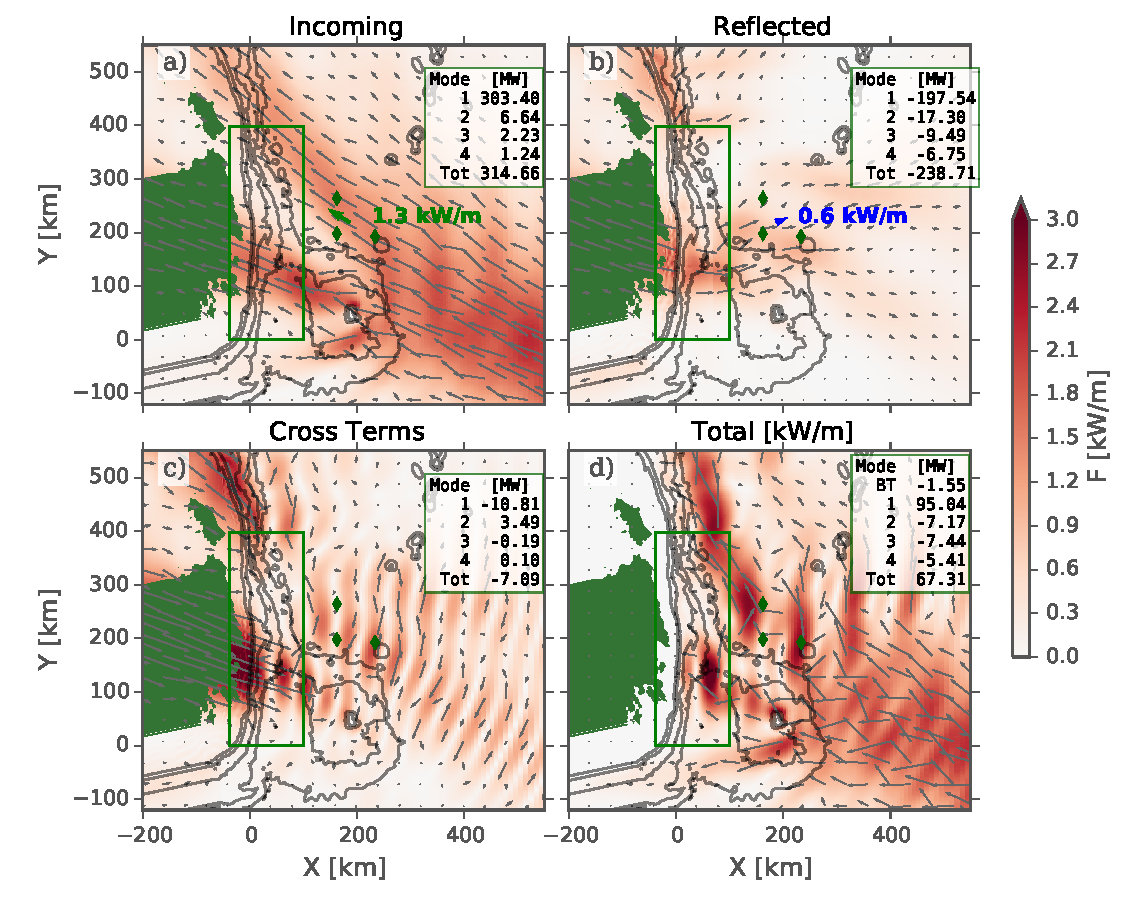
\includegraphics[width=\textwidth]{./doc/RealResponseMode1.pdf}
    \end{center}
  \end{column}

  \begin{column}{0.35\textwidth}
    \begin{itemize}
      \item In:    +314 MW (vs +408 MW w/o Tasman Rise)
      \item Cross: -  7 MW
      \item Out:   -238 MW
      \item Diss:    67 MW = 22\% (vs 40\% if we assumed Tasman Rise didn't matter)
    \end{itemize}   
    \vspace{2em}
    \footnotesize{
      (Note: slight energy imbalance -- 69 vs 67 MW -- because ``Incoming'' energy fluxes are inaccurate over shelf.)}
  \end{column}

\end{columns}
} %\end frame


\frame{\frametitle{Diffraction: Altimeter estimates}
\begin{center}
  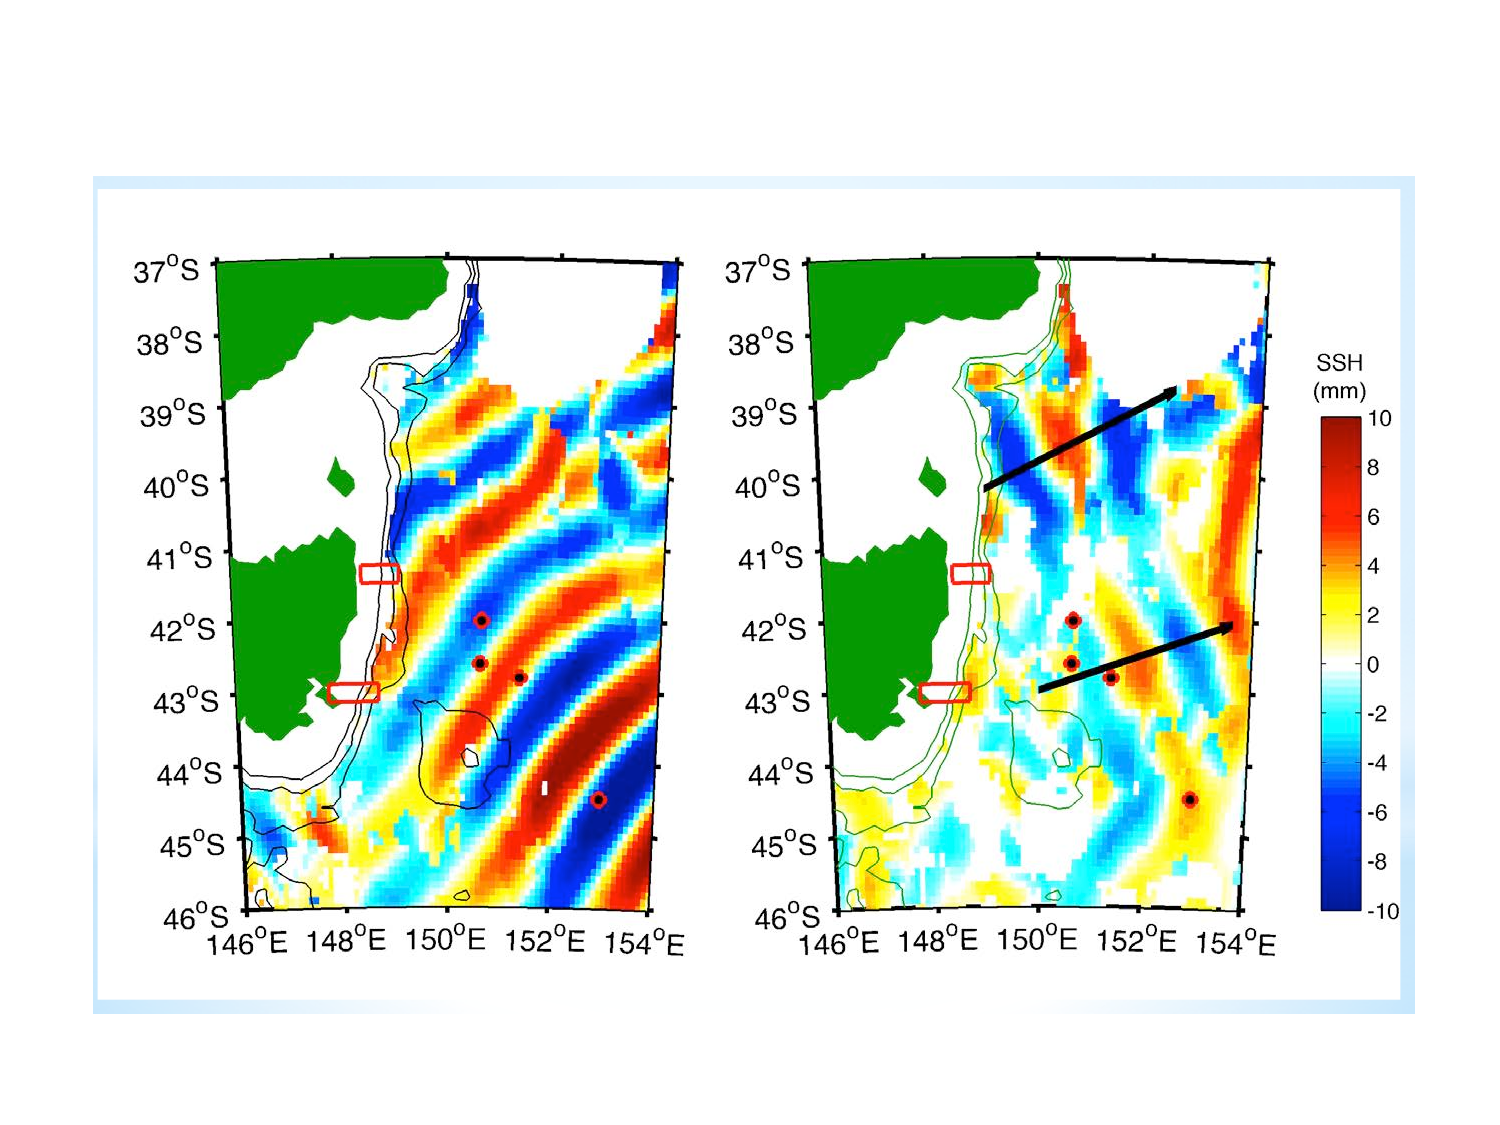
\includegraphics[width=0.8\textwidth]{./doc/ZZAltimeter.pdf}
\end{center}
\begin{itemize}
  \item Z. Zhao Altimeter measurements..
\end{itemize}
} %\end frame

\frame{\frametitle{Diffraction: Model}
\begin{center}
  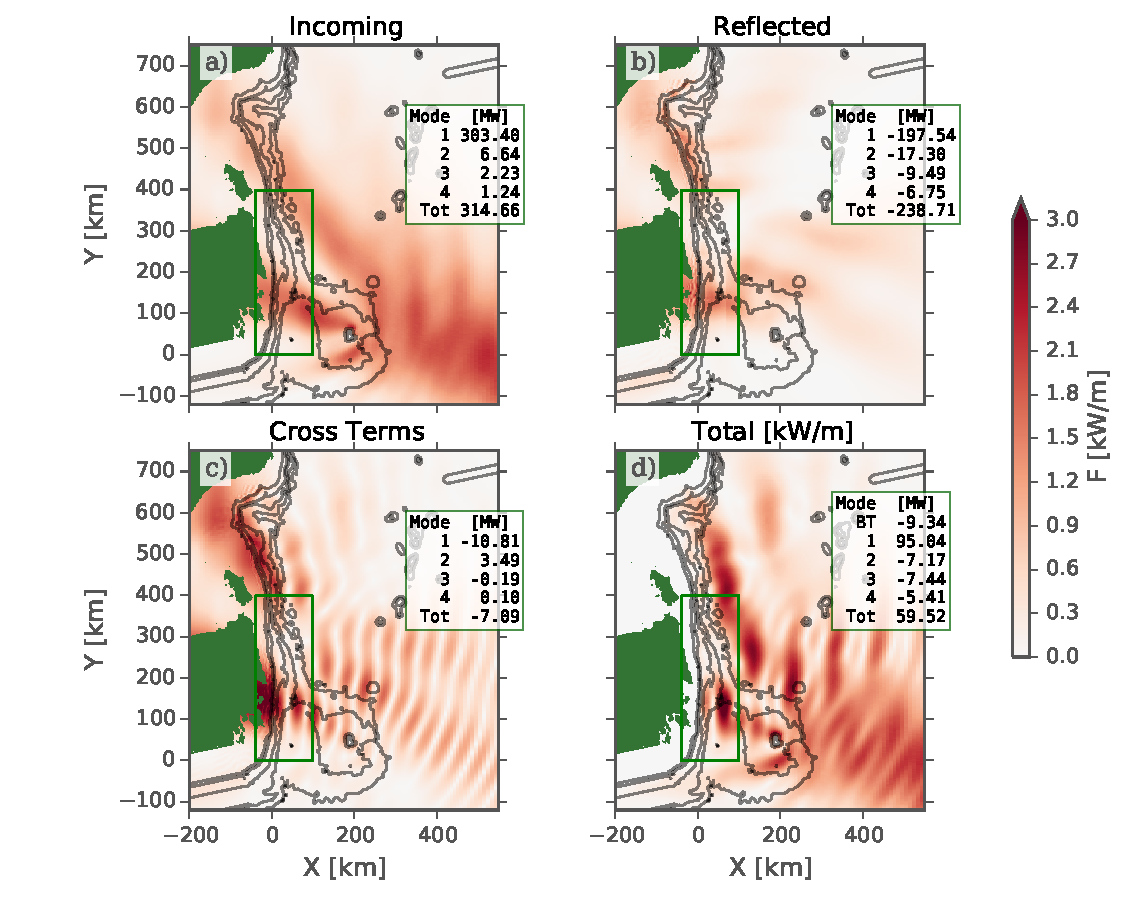
\includegraphics[width=0.62\textwidth]{./doc/RealResponseMode1Zoom.pdf}
\end{center}
} %\end frame

\frame{\frametitle{Incoming versus outgoing: Realistic}
\begin{columns}
  \begin{column}{0.45\textwidth}
    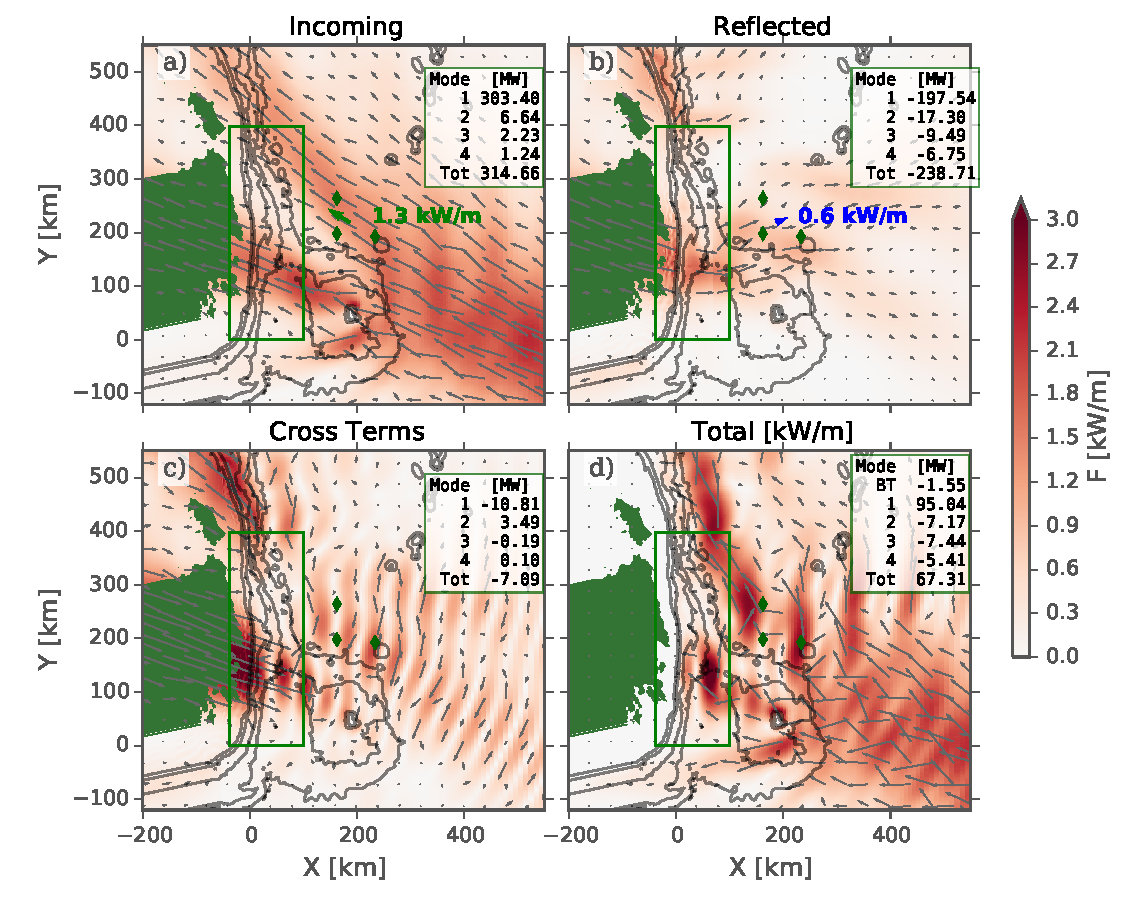
\includegraphics[width=\textwidth]{./doc/RealResponseMode1.pdf}
  \end{column}
  \begin{column}{0.55\textwidth}
    \begin{itemize}
      \item Mooring: $(1.3-0.6)/1.3\ \ \mathrm{[kW\,m^{-1}]}= 53\%$
      \item Model Mode 1 only: $(303-207)/303\ \ \mathrm{[MW]} = 30\%$
      \item Model Total: $69/315\ \ \mathrm{[MW]} = 22\%$
    \end{itemize}    
  \end{column}
\end{columns}

} %\end frame

\section{Two D comparison}
\begin{frame}
  \frametitle{Linear Model?}
  \framesubtitle{Kelly et al 2010}
  \begin{center}
    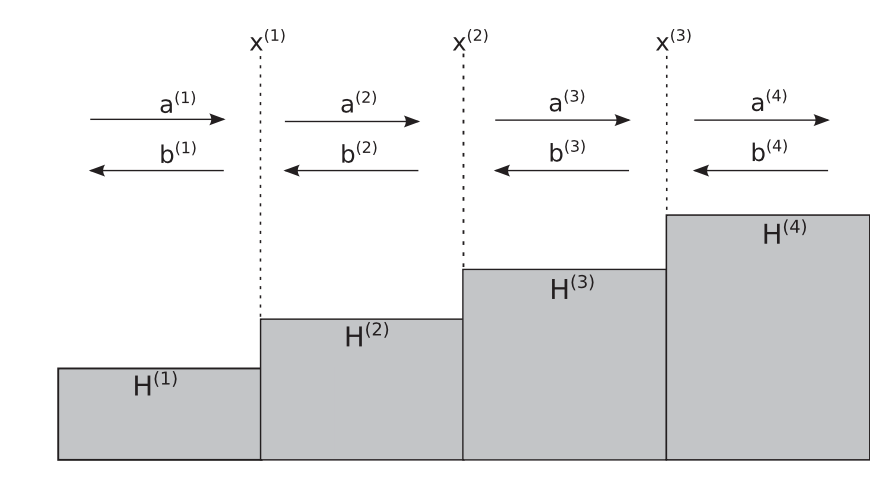
\includegraphics[width=0.45\textwidth]{doc/kellyetal13ba.png}  
    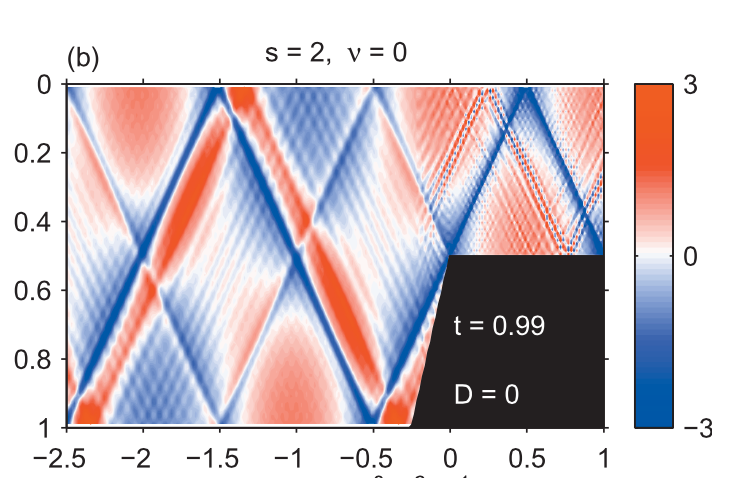
\includegraphics[width=0.45\textwidth]{doc/kellyetal13ba2.png}  
  \end{center}
  \begin{itemize}
    \item Can calculate linear response to mode-1 forcing  
    \item 2-D slices
    \item Can accommodate angular incidence.
  \end{itemize}
\end{frame}

\begin{frame}
  \frametitle{Linear Model?}
  \begin{columns}
    \begin{column}{0.2\textwidth}
      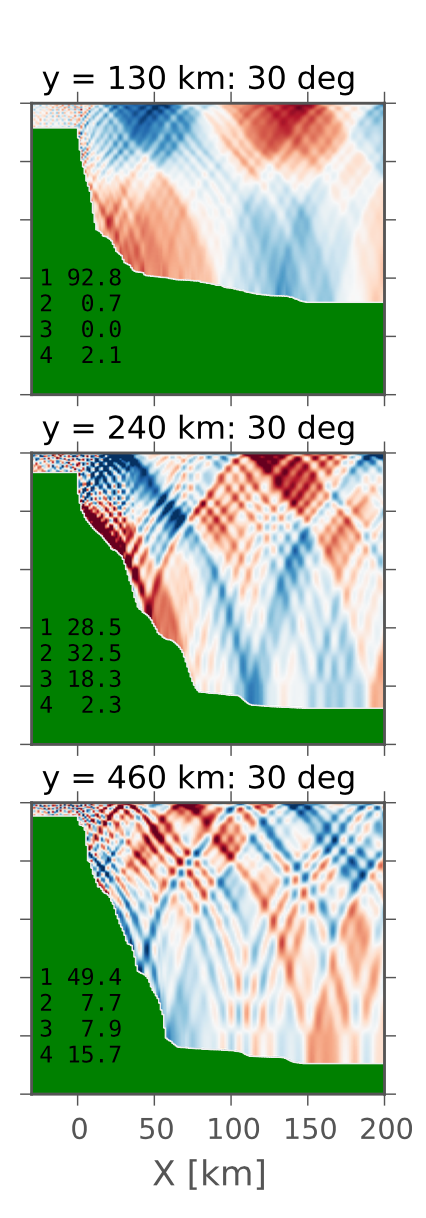
\includegraphics[width=\textwidth]{doc/MyKelly.png}  
      
    \end{column}
    \begin{column}{0.75\textwidth}
      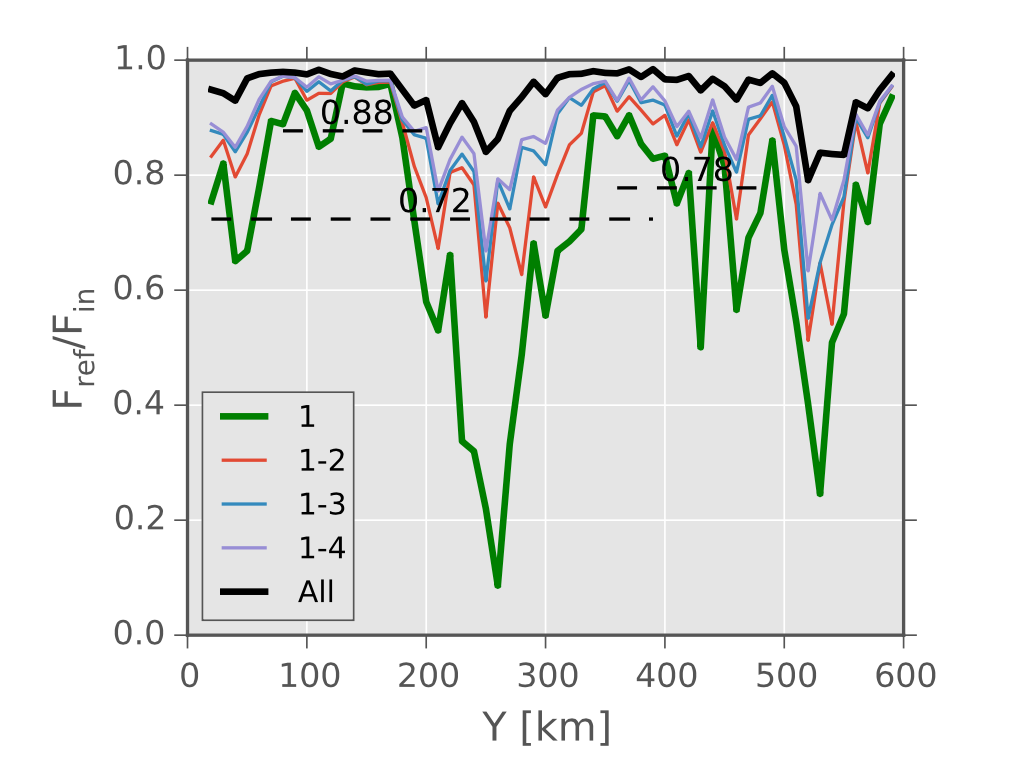
\includegraphics[width=0.6\textwidth]{doc/MyKelly2.png}  
      \begin{itemize}
        \item Model: 70\% reflected in mode-1
        \item Linear Calc: $\approx$ 80\% 
        \item Some three-dimensionality
      \end{itemize}      
    \end{column}
  \end{columns}
\end{frame}

\section{Slope Wave}
\begin{frame}

  \frametitle{Slope Wave}
  \framesubtitle{Vertically integrated energy budget}
  \begin{center}
    \includegraphics<1->[width=0.65\textwidth,trim=0 0 0 0, clip]{doc/DissReal1km03cycle20.pdf}
  \end{center}
  \begin{itemize}
    \item Alternating BT/BC conversion.
    \item $\lambda\approx 100 \ \mathrm{km}$
  \end{itemize}
\end{frame}

\frame{\frametitle{Slope Wave}
\begin{center}
  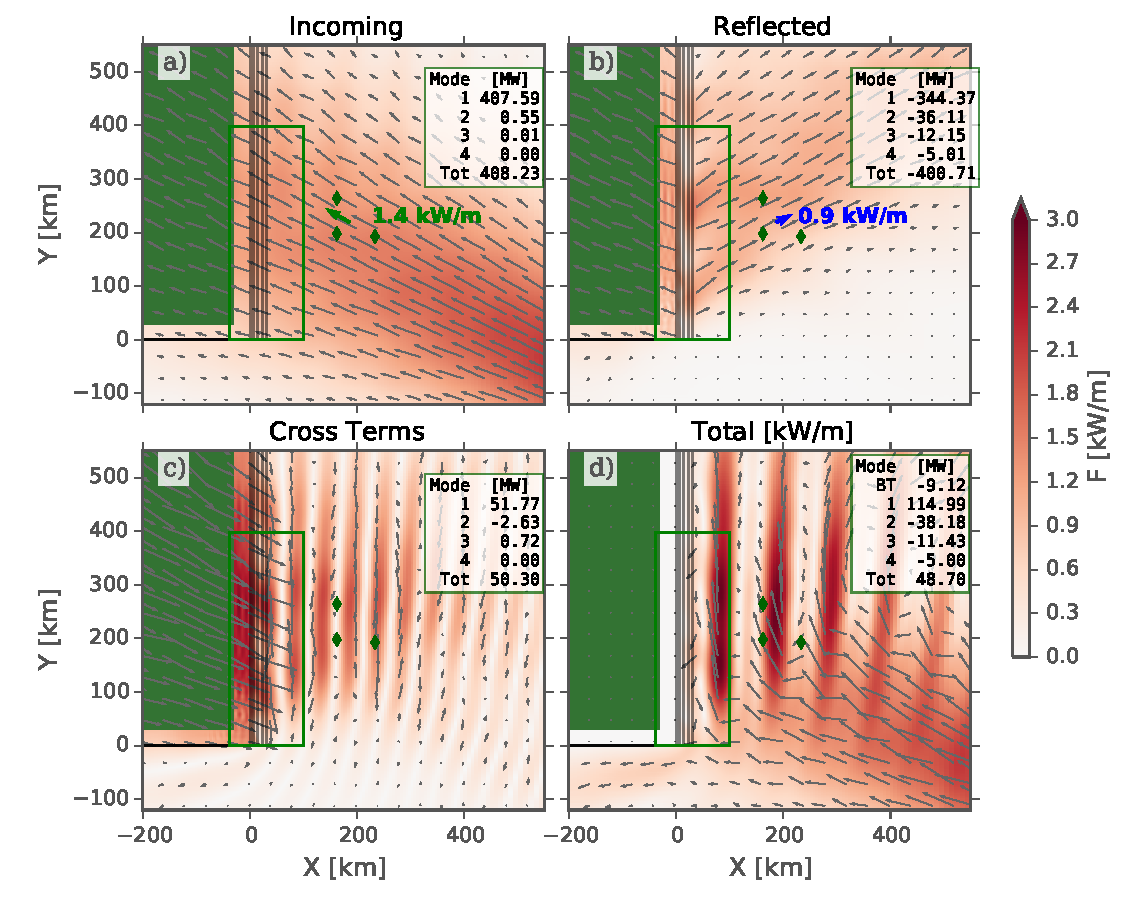
\includegraphics[width=0.62\textwidth]{./doc/ShelfResponseMode1.pdf}
\end{center}
}
\begin{frame}
  \frametitle{Slope Wave}
  \framesubtitle{Dale et. al. 2001: Super-inertial shelf waves}
  \begin{center}
     \includegraphics<1>[width=0.5\textwidth]{./doc/daleetal01a.png} 
     \includegraphics<2>[width=0.5\textwidth]{./doc/ShelfWIdthConv.png} 
  \end{center}
  \begin{itemize}
    \item<1-> \emph{Not} freely-propagating (forced)
    \item<2> ``Near-resonant'' waves depend on shelf geometry.
  \end{itemize}
\end{frame}

\section{Summary}
\begin{frame}
  \frametitle{Summary}
  \framesubtitle{What have we learned about internal tide?}
  \begin{columns}
    \begin{column}{0.5\textwidth}
      \begin{enumerate}
        \item<1-> Significant diffraction around Tasman Rise.
        \item<2-> Two-dimensional model captures some of the reflection.
        \item<3-> Super-inertial slope waves redistribute energy along slope.
      \end{enumerate}
      \onslide<4>{Complex incoming field and complex reflection implies difficult to quantify reflection experimentally.}
    \end{column}
    \begin{column}{0.5\textwidth}
      \includegraphics<1>[width=\textwidth]{doc/tasmanDiffract.png}
      \includegraphics<2>[width=\textwidth]{doc/MyKelly2.png}
      \includegraphics<3>[width=\textwidth]{doc/ShelfWIdthConv.png} 
      \includegraphics<4>[width=\textwidth]{doc/TwoWaves.pdf}
    \end{column}
    
  \end{columns}

\end{frame}

\end{document}

%%%%%%%%%%%%%%%%%%%%%%%%%%%
\section{Response}
%%%%%%%%%%%%%%%%%%%%%%%%%%%
\subsubsection{Real Response}
\frame{\frametitle{Response of real bathymetry}
  \begin{columns}
    \begin{column}{0.35\textwidth}
      \begin{itemize}
          \item 1-km resolution; idealized forcing
          \item Absolute value of energy flux (light arrows)
          \item<2-> How to get ``incoming'' versus ``reflected''?
      \end{itemize}
    \end{column}
    \begin{column}{0.65\textwidth} 
        \includegraphics<1>[width=0.95\textwidth,trim=30 10 50 20,clip]{AbsFluxReal1km03}
        \includegraphics<2->[height=0.9\textheight]{AbsFluxLastReal1km03}
    \end{column}
  \end{columns}
}% end frame

\subsubsection{Real Response}
\frame{\frametitle{Response of real bathymetry}
  \begin{columns}
    \begin{column}{0.28\textwidth}
      \begin{itemize}
          \item Diffraction around Tasman Rise (e.g., Johnston and Merrifield, 2003)
      \end{itemize}
    \end{column}
    \begin{column}{0.72\textwidth} 	  
      \includegraphics<1>[width=\textwidth]{CompareTide20RiseShelf1km03}
    \end{column}
  \end{columns}
}% end frame


%\subsection{Rise Shelf}

%\frame{\frametitle{How much reflects? Add a rise!}
%Mode 1:
%    \begin{center}
%        \includegraphics<1>[width=0.8\textwidth]{RiseShelfResponseMode1Zoom}
%    \end{center}    
%}
% end frame

%\frame{\frametitle{How much reflects? Add a rise!}
%Mode 2:
%    \begin{center}
%        \includegraphics<1>[width=0.8\textwidth]{RiseShelfResponseMode2Zoom}
%    \end{center}    
%}% end frame

%\subsection{Real bathymetry}

\subsubsection{Real shelf}
\frame{\frametitle{Modal response}
  \begin{columns}
    \begin{column}{0.38\textwidth}
      \begin{itemize}
          \item Reflection in higher modes easy
          \item Mode 1 still a mystery!  How much is coming in versus being reflected?
      \end{itemize}
    \end{column}
    \begin{column}{0.62\textwidth} 	  
      \includegraphics<1>[width=\textwidth]{ModeFluxesReal1km03}
    \end{column}
  \end{columns}
}% end frame

\frame{\frametitle{How much reflects? Real shelf}
    \begin{center}
        \includegraphics<1>[width=0.9\textwidth]{RealResponseMode1Zoom}
    \end{center}    
}% end frames
\frame{\frametitle{How much reflects? Real shelf}
            \begin{itemize}
                \item Decompose into "incoming" and "outgoing" signal.
                \item "Incoming" is from simulation without downstream topography            
            \end{itemize}
    \begin{columns}
        \begin{column}{0.4\textwidth}
            \begin{align}
                u&=u_i+u_r\\
                v&=v_i+v_r\\
                p&=p_i+p_r
            \end{align}
            \begin{align*}
                F^x &= up\\
                & = u_ip_i + u_rp_r + u_ip_r+u_rp_i\\
                    &= F^x_i + F^x_r +F^x_c
            \end{align*}            
        \end{column}
        \begin{column}{0.6\textwidth}
            \begin{center}
                \includegraphics<1>[width=0.99\textwidth]{RealResponseMode1Zoom}
            \end{center}
        \end{column}
    \end{columns}   
}% end frame

\frame{\frametitle{How much reflects? Real shelf}
            \begin{itemize}
                \item Real Shelf
                \item Energy budget from $y=0$ to $400\ \mathrm{km}$; $x<80 km$.      
                \item About 23\% of incoming energy dissipated.  
            \end{itemize}
    
            \begin{center}
                \begin{tabular}{c rrrr}
                    \hline\hline
                    Mode & Incoming & Reflected & Cross  & Total\\\hline
                    1 & 303.40 & -197.54 & -10.81 & 95.04\\ 
                    2 & 6.64 & -17.30 & 3.49 & -7.17\\ 
                    3 & 2.23 & -9.49 & -0.19 & -7.44\\ 
                    4 & 1.24 & -6.75 & 0.10 & -5.41\\ 
                    5 & 0.68 & -2.25 & 0.03 & -1.54\\ 
                    6 & 0.28 & -2.11 & 0.18 & -1.65\\ 
                    \hline 
                    Total & 314.66 & -238.71 & -7.09 & 68.86\\ \hline 
                    \end{tabular}
            \end{center}
            
}% end frame

\frame{\frametitle{How much reflects? Real shelf}
  \begin{columns}
    \begin{column}{0.35\textwidth}
      \begin{itemize}
           \item Modeled answer (0-400 km) is $F_{Reflected}/F_{Incoming} = 0.67$
           \item Can we get an accuate budget from a few moorings? 
      \end{itemize}
    \end{column}
    \begin{column}{0.65\textwidth} 
        \includegraphics[height=0.9\textheight]{AbsFluxLastReal1km03}
    \end{column}
  \end{columns}
}% end frame

\frame{\frametitle{How much reflects? Real shelf}
    \begin{columns}
        \begin{column}{0.3\textwidth}
            \begin{itemize}
                 \item Modeled answer (0-400 km) is $F_{Reflected}/F_{Incoming} = 0.67$
                \item Plane wave and proposed array gets  $F_{Reflected}/F_{Incoming}=0.42$.  
               
                \item difficult to get an accurate budget from such an array.
            \end{itemize}
        \end{column}
        \begin{column}{0.7\textwidth}
            \begin{center}      
                \includegraphics<1>[height=0.9\textheight]{JenFit.png}
                            \end{center}
        \end{column}  
    \end{columns}
}% end frame

\frame{\frametitle{How much reflects? Real Shelf}
                  \begin{center}      
                
                \includegraphics<1>[width=\textwidth]{RealResponseMode1Zoom}
            \end{center}
      
}% end frame

%%%%%%%%%%%%%%%%%%%%%%%%%%%%%%%%%%%%%%%%%%%%%%%%%%%%%%%%%%%%%%
\section{Where is dissipation}
%%%%%%%%%%%%%%%%%%%%%%%%%%%%%%%%%%%%%%%%%%%%%%%%%%%%%%%%%%%%%%

\subsubsection{What causes dissipation}
\frame{\frametitle{What causes dissipation?}
  \begin{columns}
    \begin{column}{0.38\textwidth}
      \begin{itemize}
          \item Need to resolve outer scales of breaking waves
          \item Some dissipation will be missing (i.e. shear instabilities, small scale breaking waves).
      \end{itemize}
    \end{column}
    \begin{column}{0.4\textwidth} 	
      \begin{center}
        \includegraphics<1>[height=0.85\textheight,trim=0 20 0 80,clip]{VertDissBoth}
    
      \end{center}
  
    \end{column}
  \end{columns}
}% end frame

%%%%%%%%%%%%%%%%%%%%%%%%%%%%%%%
\subsubsection{North Site}
%%%%%%%%%%%%%%%%%%%%%%%%%%%%%%%
\frame{\frametitle{Northern Site}
\centering
    \includegraphics[height=0.9\textheight,trim=50 0 0 0,clip]{VertDissFine03LinesZoom}
}% end frame
\frame{\frametitle{North Site: Onslope flow}
  \begin{columns}
    \begin{column}{0.6\textwidth}
        \includegraphics[width=\textwidth]{../Nest/SliceArbNFeat2916//Time02.png}
    \end{column}
    \begin{column}{0.4\textwidth}
    \includegraphics[width=\textwidth,trim=50 0 0 0,clip]{VertDissFine03LinesZoom}
    \end{column}
  \end{columns}
    }% 
\frame{\frametitle{North Site: Offslope flow}
  \begin{columns}
    \begin{column}{0.6\textwidth}
        \includegraphics[width=\textwidth]{../Nest/SliceArbNFeat2916//Time08.png}
    \end{column}
    \begin{column}{0.4\textwidth}
    \includegraphics[width=\textwidth,trim=50 0 0 0,clip]{VertDissFine03LinesZoom}
    \end{column}
  \end{columns}
    }% 
    


%%%%%%%%%%%%%%%%%%%%%%%%%%%%%%%%
\subsubsection{South Site}
%%%%%%%%%%%%%%%%%%%%%%%%%%%%%%%%%%
\frame{\frametitle{South Site}
  \begin{columns}
    \begin{column}{0.3\textwidth}
      \begin{itemize}
          \item Peaks and valleys "Corrugations".
      \end{itemize}
    \end{column}
    \begin{column}{0.7\textwidth}
      \includegraphics<1>[width=\textwidth,trim=30 0 20 0,clip]{VertDissFine02Zoom}     
    \end{column}
  \end{columns}
}% end frame


\frame{\frametitle{Importance of valleys: Onslope}
    \begin{columns}
        \begin{column}{0.5\textwidth}
            North Ridge:
            \includegraphics[width=\textwidth]{../Nest/SliceArbNPeak1205/Time11.png}
            
        \end{column}
        \begin{column}{0.5\textwidth}
            Valley:
            \includegraphics[width=\textwidth]{../Nest/SliceArbValley1201/Time11.png}
        \end{column}
    \end{columns}
}% end frame

\frame{\frametitle{Importance of valleys: Offslope}
    \begin{columns}
        \begin{column}{0.5\textwidth}
            North Ridge:
            \includegraphics[width=\textwidth]{../Nest/SliceArbNPeak1205/Time05.png}
            
        \end{column}
        \begin{column}{0.5\textwidth}
            Valley:
            \includegraphics[width=\textwidth]{../Nest/SliceArbValley1201/Time05.png}
        \end{column}

    \end{columns}
}% end frame

\section{Summary}

\frame{\frametitle{Summary}
\framesubtitle<1>{Internal Waves}
\framesubtitle<2->{Dissipation}
\begin{columns}
  \begin{column}{0.45\textwidth}
    \begin{itemize}
      \item<1> Beam diffracted by Tasman Rise
      \item<1> Quantifying energy fluxes in the data will require iteration with the models
      \item<2-> North: 
        \begin{itemize}
          \item<2-> Near-critical slope enhanced by deeper ``bump'' radiating energy upwards
          \item<2-> Off-slope flow dissipative
        \end{itemize}        
        \item<3> South: 
          \begin{itemize}
            \item<3> Corrugations channeling flow; channels more near-critical
            \item<3> On-slope flow dissipative.
          \end{itemize}
    \end{itemize}
  \end{column}
  \begin{column}{0.55\textwidth}
    \centering
    \includegraphics<1>[height=0.8\textheight,trim=10 0 30 0,clip]{AbsFluxLastReal1km03} 
    \includegraphics<2->[height=0.8\textheight,trim=0 20 0 80,clip]{VertDissBoth}
  \end{column}

\end{columns}
}%end frame


\end{document}

\subsection{South Site}
\frame{\frametitle{South Site}
  \begin{columns}
    \begin{column}{0.38\textwidth}
      \begin{itemize}
          \item Fine resolution (100 m x 200 m x 15 m)
          \item Peaks and valleys "Corrugations".
      \end{itemize}
    \end{column}
    \begin{column}{0.62\textwidth} 	  
      \includegraphics<1>[width=\textwidth]{SouthLineSketch}
    \end{column}
  \end{columns}
}% end frame

\subsection{South site dissipation}
Dissipation, Bottom U, and Bottom V

\frame{\frametitle{South site dissipation}
    \includegraphics<1>[width=\textwidth]{../Nest/SnapEpsZoomFine02/Snap04.png}
    \includegraphics<2>[width=\textwidth]{../Nest/SnapEpsZoomFine02/Snap05.png}
    \includegraphics<3>[width=\textwidth]{../Nest/SnapEpsZoomFine02/Snap06.png}
    \includegraphics<4>[width=\textwidth]{../Nest/SnapEpsZoomFine02/Snap07.png}
    \includegraphics<5>[width=\textwidth]{../Nest/SnapEpsZoomFine02/Snap08.png}
    \includegraphics<6>[width=\textwidth]{../Nest/SnapEpsZoomFine02/Snap09.png}
    \includegraphics<7>[width=\textwidth]{../Nest/SnapEpsZoomFine02/Snap10.png}
    \includegraphics<8>[width=\textwidth]{../Nest/SnapEpsZoomFine02/Snap11.png}
    \includegraphics<9>[width=\textwidth]{../Nest/SnapEpsZoomFine02/Snap00.png}
    \includegraphics<10>[width=\textwidth]{../Nest/SnapEpsZoomFine02/Snap01.png}
    \includegraphics<11>[width=\textwidth]{../Nest/SnapEpsZoomFine02/Snap02.png}
    \includegraphics<12>[width=\textwidth]{../Nest/SnapEpsZoomFine02/Snap03.png}
}% end frame


\frame{\frametitle{South Site}
  \begin{columns}
    \begin{column}{0.38\textwidth}
      \begin{itemize}
          \item Fine resolution (100 m x 200 m x 15 m)
          \item Peaks and valleys "Corrugations".
      \end{itemize}
    \end{column}
    \begin{column}{0.62\textwidth} 	  
      \includegraphics<1>[width=\textwidth]{SouthLineSketch}
    \end{column}
  \end{columns}
}% end frame

% site
% lines


\frame{\frametitle{Valley}
    \includegraphics<1>[width=0.65\textwidth]{../Nest/SliceArbValley1201//Time04.png}
    \includegraphics<2>[width=0.65\textwidth]{../Nest/SliceArbValley1201//Time05.png}
    \includegraphics<3>[width=0.65\textwidth]{../Nest/SliceArbValley1201//Time06.png}
    \includegraphics<4>[width=0.65\textwidth]{../Nest/SliceArbValley1201//Time07.png}
    \includegraphics<5>[width=0.65\textwidth]{../Nest/SliceArbValley1201//Time08.png}
    \includegraphics<6>[width=0.65\textwidth]{../Nest/SliceArbValley1201//Time09.png}
    \includegraphics<7>[width=0.65\textwidth]{../Nest/SliceArbValley1201//Time10.png}
    \includegraphics<8>[width=0.65\textwidth]{../Nest/SliceArbValley1201/Time11.png}
    \includegraphics<9>[width=0.65\textwidth]{../Nest/SliceArbValley1201/Time00.png}
    \includegraphics<10>[width=0.65\textwidth]{../Nest/SliceArbValley1201/Time01.png}
    \includegraphics<11>[width=0.65\textwidth]{../Nest/SliceArbValley1201/Time02.png}
    \includegraphics<12>[width=0.65\textwidth]{../Nest/SliceArbValley1201/Time03.png}
}% end frame

\frame{\frametitle{North Peak}
    \includegraphics<1>[width=0.65\textwidth]{../Nest/SliceArbNPeak1205//Time04.png}
    \includegraphics<2>[width=0.65\textwidth]{../Nest/SliceArbNPeak1205//Time05.png}
    \includegraphics<3>[width=0.65\textwidth]{../Nest/SliceArbNPeak1205//Time06.png}
    \includegraphics<4>[width=0.65\textwidth]{../Nest/SliceArbNPeak1205//Time07.png}
    \includegraphics<5>[width=0.65\textwidth]{../Nest/SliceArbNPeak1205//Time08.png}
    \includegraphics<6>[width=0.65\textwidth]{../Nest/SliceArbNPeak1205//Time09.png}
    \includegraphics<7>[width=0.65\textwidth]{../Nest/SliceArbNPeak1205//Time10.png}
    \includegraphics<8>[width=0.65\textwidth]{../Nest/SliceArbNPeak1205/Time11.png}
    \includegraphics<9>[width=0.65\textwidth]{../Nest/SliceArbNPeak1205/Time00.png}
    \includegraphics<10>[width=0.65\textwidth]{../Nest/SliceArbNPeak1205/Time01.png}
    \includegraphics<11>[width=0.65\textwidth]{../Nest/SliceArbNPeak1205/Time02.png}
    \includegraphics<12>[width=0.65\textwidth]{../Nest/SliceArbNPeak1205/Time03.png}
}% end frame


\frame{\frametitle{Importance of valleys "flood"}
    \begin{columns}
        \begin{column}{0.33\textwidth}
            North Ridge:
            \includegraphics[width=\textwidth]{../Nest/SliceArbNPeak1205/Time11.png}
            
        \end{column}
        \begin{column}{0.33\textwidth}
            Valley:
            \includegraphics[width=\textwidth]{../Nest/SliceArbValley1201/Time11.png}
        \end{column}
        \begin{column}{0.33\textwidth}
            South Ridge:
            \includegraphics[width=\textwidth]{../Nest/SliceArbSPeak1179/Time11.png}

        \end{column}

    \end{columns}

}% end frame

\frame{\frametitle{Importance of valleys "ebb"}
    \begin{columns}
        \begin{column}{0.33\textwidth}
            North Ridge:
            \includegraphics[width=\textwidth]{../Nest/SliceArbNPeak1205/Time05.png}
            
        \end{column}
        \begin{column}{0.33\textwidth}
            Valley:
            \includegraphics[width=\textwidth]{../Nest/SliceArbValley1201/Time05.png}
        \end{column}
        \begin{column}{0.33\textwidth}
            South Ridge:
            \includegraphics[width=\textwidth]{../Nest/SliceArbSPeak1179/Time05.png}

        \end{column}

    \end{columns}

}% end frame

\frame{\frametitle{Importance of valleys "flood"}
    \begin{columns}
        \begin{column}{0.33\textwidth}
            North Ridge:
            \includegraphics[width=\textwidth]{../Nest/SliceArbNPeak1205/Time11.png}
            
        \end{column}
        \begin{column}{0.33\textwidth}
            Valley:
            \includegraphics[width=\textwidth]{../Nest/SliceArbValley1201/Time11.png}
        \end{column}
        \begin{column}{0.33\textwidth}
            South Ridge:
            \includegraphics[width=\textwidth]{../Nest/SliceArbSPeak1179/Time11.png}

        \end{column}

    \end{columns}
    Mechanism:
    \begin{itemize}
        \item upslope flow turbulent 
        \item downslope largely laminar
        \item valleys more near critical: enhanced near bottom velocity
    \end{itemize}


}% end frame
\section{North Site}

\frame{\frametitle{Northern Site}
    \includegraphics[width=\textwidth]{VertDissFine03LinesZoom}
}% end frame

\frame{\frametitle{North Site}
    \includegraphics<1>[width=0.999\textwidth]{../Nest/SnapEpsZoomFine03//Snap09.png}
    \includegraphics<2>[width=0.999\textwidth]{../Nest/SnapEpsZoomFine03//Snap10.png}
    \includegraphics<3>[width=0.999\textwidth]{../Nest/SnapEpsZoomFine03//Snap11.png}
    \includegraphics<4>[width=0.999\textwidth]{../Nest/SnapEpsZoomFine03//Snap00.png}
    \includegraphics<5>[width=0.999\textwidth]{../Nest/SnapEpsZoomFine03//Snap01.png}
    \includegraphics<6>[width=0.999\textwidth]{../Nest/SnapEpsZoomFine03//Snap02.png}
    \includegraphics<7>[width=0.999\textwidth]{../Nest/SnapEpsZoomFine03//Snap03.png}
    \includegraphics<8>[width=0.999\textwidth]{../Nest/SnapEpsZoomFine03/Snap04.png}
    \includegraphics<9>[width=0.999\textwidth]{../Nest/SnapEpsZoomFine03/Snap05.png}
    \includegraphics<10>[width=0.999\textwidth]{../Nest/SnapEpsZoomFine03/Snap06.png}
    \includegraphics<11>[width=0.999\textwidth]{../Nest/SnapEpsZoomFine03/Snap07.png}
    \includegraphics<12>[width=0.999\textwidth]{../Nest/SnapEpsZoomFine03/Snap08.png}
    \includegraphics<13>[width=0.999\textwidth]{../Nest/SnapEpsZoomFine03/Snap09.png}
    \includegraphics<14>[width=0.999\textwidth]{../Nest/SnapEpsZoomFine03/Snap10.png}
    \includegraphics<15>[width=0.999\textwidth]{../Nest/SnapEpsZoomFine03/Snap11.png}
    \includegraphics<16>[width=0.999\textwidth]{../Nest/SnapEpsZoomFine03/Snap00.png}
}% end frame

\frame{\frametitle{North Site}
    \includegraphics<1>[width=0.65\textwidth]{../Nest/SliceArb032916//Time09.png}
    \includegraphics<2>[width=0.65\textwidth]{../Nest/SliceArb032916//Time10.png}
    \includegraphics<3>[width=0.65\textwidth]{../Nest/SliceArb032916//Time11.png}
    \includegraphics<4>[width=0.65\textwidth]{../Nest/SliceArb032916//Time00.png}
    \includegraphics<5>[width=0.65\textwidth]{../Nest/SliceArb032916//Time01.png}
    \includegraphics<6>[width=0.65\textwidth]{../Nest/SliceArb032916//Time02.png}
    \includegraphics<7>[width=0.65\textwidth]{../Nest/SliceArb032916//Time03.png}
    \includegraphics<8>[width=0.65\textwidth]{../Nest/SliceArb032916/Time04.png}
    \includegraphics<9>[width=0.65\textwidth]{../Nest/SliceArb032916/Time05.png}
    \includegraphics<10>[width=0.65\textwidth]{../Nest/SliceArb032916/Time06.png}
    \includegraphics<11>[width=0.65\textwidth]{../Nest/SliceArb032916/Time07.png}
    \includegraphics<12>[width=0.65\textwidth]{../Nest/SliceArb032916/Time08.png}
    \includegraphics<13>[width=0.65\textwidth]{../Nest/SliceArb032916/Time09.png}
    \includegraphics<14>[width=0.65\textwidth]{../Nest/SliceArb032916/Time10.png}
    \includegraphics<15>[width=0.65\textwidth]{../Nest/SliceArb032916/Time11.png}
    \includegraphics<16>[width=0.65\textwidth]{../Nest/SliceArb032916/Time00.png}
}% end frame
\frame{\frametitle{North Site: Onslope flow}
    \includegraphics[width=0.65\textwidth]{../Nest/SliceArb032916//Time02.png}
    }% 
\frame{\frametitle{North Site: Offslope flow}
    \includegraphics[width=0.65\textwidth]{../Nest/SliceArb032916//Time08.png}
    }% end frame

\frame{\frametitle{Recipe?}
    \begin{columns}
        \begin{column}{0.4\textwidth}
            \begin{itemize}
                \item Critical region
                \item upslope supercrtical: during onslope?
                \item upslope subcritical: during offslope?
                \item \emph{Gemmrich and Klymak, 2015} looking at part of this.
            \end{itemize}
                
        \end{column}
        \begin{column}{0.6\textwidth}
            \includegraphics[width=\textwidth]{../Nest/SliceArb032916//Time08.png}
        \end{column}
    \end{columns}
}% end frame

\end{document}


%\frame{\frametitle{Movie!}
%
%\begin{center}
%\movie[autostart,loop,width=3.8in,height=2.85in]{}{Cv1300Rough3D.mov}
%
%\end{center}
%}

\clearpage
\end{document}
